\chapter{약한 장, 중력파와 작용 원리}

일반상대성이론의 정확한 방정식은 비선형이며, 물리 문제를 하나도 풀기 전에 성분 형태만으로도 다루기 벅찰 수 있다. 이 강좌의 마지막 강의에서는 원리와 계산을 분리해 보는 편이 낫다. 중력장이 약할 때 아인슈타인 방정식이 어떤 형태가 되는지 묻고, 그 근사에 포함된 파동을 확인한 다음, 완전한 장 방정식이 놀라울 만큼 간결한 작용 원리 안에 어떻게 들어가는지 살펴보며 마무리하겠다.

세 가지 질문을 중심으로 논의를 진행한다. 약한 중력장이란 무엇인가? 정확한 이론은 비선형인데 약한 장 이론은 왜 선형인가? 그리고 중력파를 단순한 좌표의 물결과 구별해 주는 물리적 효과는 무엇인가?

\section{평형 기하의 작은 교란}

약함은 근사 방법의 한 조건이다. 무차원 섭동의 크기가 \(\epsilon\ll1\)이면 그 제곱의 크기는 \(\epsilon^2\)이므로, 1차 계산에서는 후자를 일관되게 버린다. 익숙한 예로는 평형 상태 주위에서 작은 진동을 하는 역학계가 있다. 정확한 방정식은 비선형일 수 있지만, 진동이 충분히 작으면 선형 방정식을 따른다.

중력의 경우 평형 배경은 물질이 없는 평탄한 시공간이다. 아인슈타인의 진공 방정식에서 시작하자.
\begin{equation}
 R_{\mu\nu}-\frac12 g_{\mu\nu}R=0.
 \label{eq:l10-vacuum-einstein}
\end{equation}
4차원에서 양변의 대각합을 취하면
\begin{equation}
 g^{\mu\nu}
 \left(R_{\mu\nu}-\frac12 g_{\mu\nu}R\right)
 =R-2R=-R=0,
\end{equation}
따라서 진공 방정식은 다음과 동치다.
\begin{equation}
 R_{\mu\nu}=0.
 \label{eq:l10-ricci-flat}
\end{equation}

\begin{figure}[htbp]
\centering
\includegraphics[width=0.68\textwidth]{lecture_10_figure_02.png}
\caption{약한 장 논의를 시작할 때 제시한 진공 방정식 \(R_{\mu\nu}=0\).}
\lectureframe{00:03:11}
\end{figure}

여기서 평형이란 시간에 따라 변하지 않는 무원천 해를 뜻한다. 평탄한 시공간은 이런 해 가운데 가장 단순하다. 단, 반드시 짚고 넘어갈 점이 있다. 평탄하다는 것은 모든 좌표계에서 계량 성분이 특정 행렬과 같다는 뜻이 아니다. 관성 좌표계를 선택하면 다음과 같이 쓸 수 있다는 뜻이다.
\begin{equation}
 g_{\mu\nu}=\eta_{\mu\nu}.
\end{equation}
기하와 그 기하를 기술하는 좌표의 차이가 곧 핵심적인 미묘함으로 떠오를 것이다.

이제 쌍성계처럼 격렬한 원천을 생각해 보자. 원천 가까이에서는 장이 강할 수 있지만, 원천에서 멀어지면 섭동은 퍼져 나가면서 작아진다. 적절한 좌표계에서는 계량을 다음과 같이 쓸 수 있다.
\begin{equation}
 g_{\mu\nu}(x)=\eta_{\mu\nu}+h_{\mu\nu}(x),
 \qquad |h_{\mu\nu}|\ll1.
 \label{eq:weak-split}
\end{equation}
섭동 \(h_{\mu\nu}\)은 시공간의 네 좌표 모두에 의존할 수 있다. 약한 장 근사에서는 1차를 넘는 항들을 무시한다.

\section{1차에서 남는 것}

완전한 리치 텐서는 이 단계에서 활용하기에 너무 복잡하다. 구조만 보면 충분하다. 크리스토펠 기호에는 역계량과 계량의 1차 미분이 들어가며, 곡률에는 크리스토펠 기호의 미분과 크리스토펠 기호 두 개의 곱이 들어간다.
\begin{equation}
 \Gamma\sim\frac12 g^{-1}\partial g,
 \qquad
 R\sim\partial\Gamma+\Gamma\Gamma.
 \label{eq:curvature-skeleton}
\end{equation}

\begin{figure}[htbp]
\centering
\includegraphics[width=0.84\textwidth]{lecture_10_figure_03.png}
\caption{약한 장 분해와 개략적인 구성 \(R\sim\partial\Gamma+\Gamma\Gamma\). 이 표기법은 모든 지표를 전개하지 않고도 \(h\)의 차수를 드러낸다.}
\lectureframe{00:10:17}
\end{figure}

역계량은 다음 관계에서 구한다.
\(g^{\mu\alpha}g_{\alpha\nu}=\delta^\mu{}_\nu\). 1차까지 쓰면
\begin{equation}
 g^{\mu\nu}=\eta^{\mu\nu}-h^{\mu\nu}+O(h^2),
 \label{eq:inverse-weak}
\end{equation}
여기서 \(h\)의 지표는 배경 계량으로 올린다. 관성 좌표계에서는 배경 계량이 상수이므로
\begin{equation}
 \partial_\alpha\eta_{\mu\nu}=0,
\end{equation}
따라서
\begin{equation}
 \partial_\alpha g_{\mu\nu}
 =\partial_\alpha h_{\mu\nu}.
\end{equation}
결과적으로
\begin{equation}
\begin{aligned}
 \Gamma&=O(\partial h),\\
 R_{\mu\nu}
 &=O(\partial\partial h)+O\bigl((\partial h)^2\bigr)\\
 &\quad+O(h\,\partial\partial h).
\end{aligned}
 \label{eq:ricci-orders}
\end{equation}

\begin{figure}[htbp]
\centering
\includegraphics[width=0.84\textwidth]{lecture_10_figure_04.png}
\caption{칠판에 전개한 역계량과 \(\partial\eta=0\)라는 관찰. 선도 차수에는 \(h_{\mu\nu}\)의 미분만 남는다.}
\lectureframe{00:11:55}
\end{figure}

식~\eqref{eq:ricci-orders}의 마지막 두 항은 섭동의 제곱에 비례하므로 생략한다. 따라서 진공 방정식은 \(h_{\mu\nu}\)의 2차 미분을 포함하는 선형 방정식이 된다. 선형화란 바로 이런 뜻이다. 아인슈타인의 정확한 이론이 선형이라는 주장이 아니다.

\begin{classroomqa}
\audiencequestion{곡률 텐서에는 지표가 네 개 있고 리치 텐서에는 두 개 있다. 두 미분에 이미 지표가 붙어 있고 \(h_{\mu\nu}\)에도 지표가 두 개 더 있다면, 지표 수는 어떻게 맞는가?}
\lecturerresponse{리치 텐서는 곡률 텐서의 지표 한 쌍을 축약해 얻는다. 이 축약에 쓰는 계량은 자유 지표 두 개를 남기며, 이 지표는 \(R_{\mu\nu}\)에 붙은 지표 두 개와 정확히 일치한다. 기호식 \(\partial\partial h\)은 이러한 축약을 생략한 차수 표시이지, 지표를 모두 쓴 완전한 식은 아니다.
\lecturetimestamp{00:18:45--00:19:53}}
\end{classroomqa}

\begin{classroomqa}
\audiencequestion{역계량으로 축약하면 \(h\,\partial^2h\) 같은 항이 생기는가? 생긴다면 왜 무시해도 되는가?}
\lecturerresponse{그렇다. \(g^{-1}\)을 \(\eta^{-1}-h+\cdots\)로 바꾸면 1차 항 \(\eta^{-1}\partial^2h\)과 \(h\)이 하나 더 포함된 보정항들이 생긴다. 후자는 2차 항이다. 같은 규칙에 따라 \(h\,\partial h\), \(h\,\partial^2h\), \((\partial h)^2\)도 버린다. 섭동의 거듭제곱을 하나만 남기는 것이 바로 여기서 취하는 근사다.
\lecturetimestamp{00:19:55--00:21:14}}
\end{classroomqa}

\section{방정식이 파동처럼 보이는 이유}

2차 미분을 포함하는 장 방정식은 자연스럽게 파동 전파를 떠올리게 한다. \(z\)축을 따라 움직이는 스칼라 함수의 경우, 기본적인 파동 방정식은 다음과 같다.
\begin{equation}
 \left(\partial_t^2-\partial_z^2\right)\phi=0,
\end{equation}
그 해에는 임의의 오른쪽 진행 및 왼쪽 진행 파형이 포함된다.
\begin{equation}
 \phi(z,t)=f(z-t)+g(z+t).
\end{equation}
공간 차원이 3인 경우에는 같은 방정식이 다음과 같다.
\begin{equation}
 \left(\partial_t^2-\nabla^2\right)\phi=0.
\end{equation}
이 방정식은 선형이므로 중첩이 가능하다. 해 두 개의 합도 또 하나의 해다.

중력은 스칼라장이 아니다. 섭동은 텐서 성분을 가지며, 방정식 \(R_{\mu\nu}=0\)은 처음에는 여러 성분 방정식을 제공하는 것처럼 보인다. 하지만 이 방정식들이 모두 독립인 것은 아니다. 일부는 구속 조건이고, 일부는 좌표 자유도에 해당한다. 이는 맥스웰 이론과 유사하다. 맥스웰 이론에서도 일련의 장 방정식 가운데 결국 물리적인 횡파만 남는다.

적절한 좌표 조건을 부과하면 복사 성분은 보통의 파동 방정식을 만족한다.
\begin{equation}
 \Box h_{\mu\nu}=0,
 \qquad
 \Box=\eta^{\alpha\beta}\partial_\alpha\partial_\beta.
 \label{eq:linear-wave}
\end{equation}
\(\Box\) 안의 부호는 부호 규약에 따라 달라지지만, 방정식의 내용은 변하지 않는다. 섭동은 광원뿔을 따라 전파된다.

\section{좌표의 흔들림은 중력파가 아니다}

선형화 방정식의 모든 해를 물리적인 파동으로 받아들이기 전에, 좌표에 관한 주의 사항을 다시 살펴보자. 평탄한 공간도 곡선 좌표선으로 기술할 수 있다. 이때 공간의 곡률은 여전히 0인데도 계량 성분은 직교좌표에서의 값과 달라진다.

칠판에서 바로 예를 볼 수 있다. 평평한 칠판에 직교좌표를 직선으로 그린 뒤 다음과 같이 쓰자.
\begin{equation}
 ds^2=\delta_{mn}\,dx'^m dx'^n.
\end{equation}
이제 같은 점들을 약간 물결치는 좌표로 다시 표시하자.
\begin{equation}
 x'^m=x^m+f^m(x).
 \label{eq:small-coordinate-change}
\end{equation}
미분은 다음과 같이 바뀐다.
\begin{equation}
 dx'^m=dx^m+\partial_n f^m\,dx^n.
\end{equation}
이를 선요소에 대입하고 \(f\)의 1차 항까지만 남기면
\begin{align}
 ds^2
 &=\delta_{mn}dx^m dx^n\\
 &\quad+\left(\partial_m f_n+\partial_n f_m\right)dx^m dx^n
 +O(f^2).
\end{align}
따라서 다음 형태의 겉보기 섭동은
\begin{equation}
 h_{mn}=\partial_m f_n+\partial_n f_m
 \label{eq:pure-gauge}
\end{equation}
새로운 기하를 전혀 나타내지 않을 수 있다. 물결치는 좌표로 기술한 평탄한 공간일 뿐이다.

\begin{figure}[htbp]
\centering
\includegraphics[width=0.84\textwidth]{lecture_10_figure_05.png}
\caption{칠판에 전개한 좌표의 물결 계산. 좌표를 조금 다시 잡으면 칠판은 여전히 평탄한데도 겉보기에 작은 \(h_{mn}\)이 생긴다.}
\lectureframe{00:27:54}
\end{figure}

식~\eqref{eq:pure-gauge}은 좌표 자유도, 즉 게이지 자유도의 선형화된 형태다. 이런 가짜 섭동을 없애려면 추가 조건이 필요하다. 여기서는 자세한 게이지 대수를 다루지 않는다. 중요한 것은 그 역할이다. 게이지 조건은 곡률의 변화를 보존하면서 기술 방식의 변화만 제거한다. 좌표 자유도와 구속 방정식을 고려하고 나면 물리적 내용은 서로 독립인 두 개의 파동 편광으로 줄어든다.

\begin{figure}[htbp]
\centering
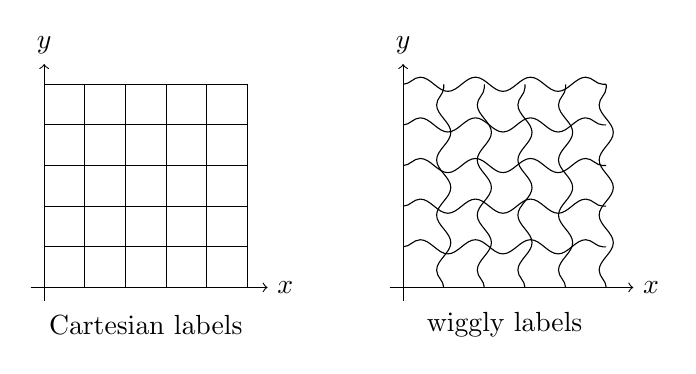
\begin{tikzpicture}[scale=0.86]
\begin{scope}
\draw[->] (-0.2,0) -- (3.3,0) node[right] {$x$};
\draw[->] (0,-0.2) -- (0,3.3) node[above] {$y$};
\foreach \u in {0.6,1.2,1.8,2.4,3.0}{
  \draw (\u,0) -- (\u,3.0);
  \draw (0,\u) -- (3.0,\u);
}
\node at (1.5,-0.55) {Cartesian labels};
\end{scope}
\begin{scope}[xshift=5.3cm]
\draw[->] (-0.2,0) -- (3.4,0) node[right] {$x$};
\draw[->] (0,-0.2) -- (0,3.3) node[above] {$y$};
\foreach \u in {0.6,1.2,1.8,2.4,3.0}{
  \draw[decorate,decoration={snake,amplitude=0.09cm,segment length=0.7cm}]
    (\u,0) -- (\u,3.0);
  \draw[decorate,decoration={snake,amplitude=0.09cm,segment length=0.7cm}]
    (0,\u) -- (3.0,\u);
}
\node at (1.5,-0.55) {wiggly labels};
\end{scope}
\end{tikzpicture}
\caption{기하는 평탄한 채로 좌표 격자만 바뀐다. 계량 성분만으로는 섭동이 물리적인지 판단할 수 없다.}
\end{figure}

\section{z축을 따라 진행하는 파동}

양의 \(z\) 방향으로 진행하는 평면파를 택하자. 위상은 다음과 같이 쓸 수 있다.
\begin{equation}
 k(z-t),
\end{equation}
그러면 한 대표 성분은 다음 형태를 갖는다.
\begin{equation}
 h_{\mu\nu}(z,t)
 =h_{\mu\nu}^{(0)}\sin k(z-t).
 \label{eq:plane-wave}
\end{equation}
위상이 일정한 면은 \(z-t=\text{constant}\)를 만족하므로, 전파 속도는 빛의 속도다.

횡방향-무흔적 표현에서는 시간 지표나 \(z\) 지표가 들어간 성분이 사라진다.
\begin{equation}
 h_{0\mu}=0,
 \qquad
 h_{z\mu}=0.
 \label{eq:tt-transverse}
\end{equation}
\(x\)-\(y\) 블록만 남는다. 이 블록은 대칭이고 무흔적이며,
\begin{equation}
 h_{xy}=h_{yx},
 \qquad
 h_{xx}+h_{yy}=0.
 \label{eq:tt-trace}
\end{equation}

\begin{figure}[htbp]
\centering
\includegraphics[width=0.84\textwidth]{lecture_10_figure_06.png}
\caption{\(z\) 방향으로 진행하는 파동을 횡방향 평면들의 층으로 나타냈다. 남는 \(x\)-\(y\) 진폭은 \(h_{xx}+h_{yy}=0\)을 만족한다.}
\lectureframe{00:43:36}
\end{figure}

따라서 서로 독립인 패턴은 두 가지다. \(i,j\in\{x,y\}\)에 대해 이를 다음과 같이 나타낼 수 있다.
\begin{equation}
 h^{\mathrm{TT}}_{ij}(z,t)
 =
 \begin{pmatrix}
 h_+ & h_\times\\
 h_\times & -h_+
 \end{pmatrix}
 \sin k(z-t).
 \label{eq:polarization-matrix}
\end{equation}
대각 성분 패턴을 플러스 편광이라고 한다. 비대각 성분 패턴은 크로스 편광이라고 한다. 횡축을 \(45^\circ\)만큼 회전하면 한 패턴이 다른 패턴으로 바뀌며, 임의의 선편광 파동은 두 패턴의 중첩이다. 이 이론에는 이 밖에 독립적인 편광이 없다.

\begin{figure}[htbp]
\centering
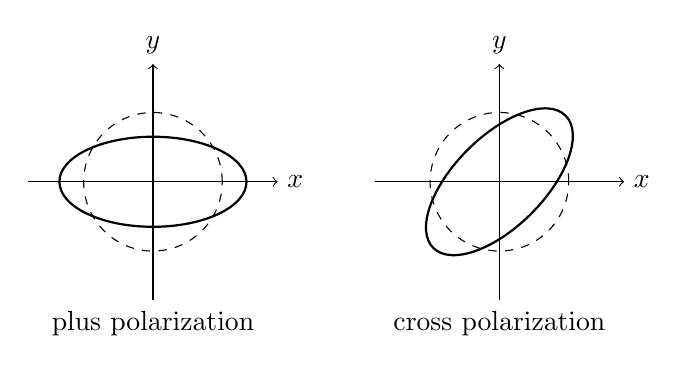
\begin{tikzpicture}[scale=0.88]
\begin{scope}
\draw[->] (-1.8,0) -- (1.8,0) node[right] {$x$};
\draw[->] (0,-1.7) -- (0,1.7) node[above] {$y$};
\draw[dashed] (0,0) circle (1.0);
\draw[thick] (0,0) ellipse (1.35 and 0.65);
\node at (0,-2.05) {plus polarization};
\end{scope}
\begin{scope}[xshift=5.0cm]
\draw[->] (-1.8,0) -- (1.8,0) node[right] {$x$};
\draw[->] (0,-1.7) -- (0,1.7) node[above] {$y$};
\draw[dashed] (0,0) circle (1.0);
\draw[thick,rotate=45] (0,0) ellipse (1.35 and 0.65);
\node at (0,-2.05) {cross polarization};
\end{scope}
\end{tikzpicture}
\caption{반주기 동안 한 횡방향은 늘어나고 수직 방향은 줄어든다. 반주기가 더 지나면 변형 방향이 반대로 바뀐다.}
\end{figure}

\section{계량 성분에서 물리적 변형률까지}

\(z\)와 \(t\)을 고정하고 횡단면을 살펴보자. 순수한 플러스 파동의 경우
\begin{equation}
 ds_\perp^2
 =(1+h_{xx})\,dx^2+(1-h_{xx})\,dy^2.
 \label{eq:transverse-distance}
\end{equation}
\(h_{xx}>0\)일 때 \(x\) 방향의 고정된 좌표 간격은 고유 길이가 약간 늘어나고, 이에 대응하는 \(y\) 방향 간격은 약간 줄어든다. 반주기 뒤에는 \(h_{xx}\)의 부호가 바뀌어 늘고 줄어드는 방향도 뒤바뀐다. 정사각형은 가로로 늘어나고 세로로 줄었다가, 다음에는 가로로 줄고 세로로 늘어난다. 크로스 편광에서는 같은 변화가 \(45^\circ\) 회전한 축을 따라 일어난다.

처음 길이가 \(L\)인 막대는 1차 근사에서 다음만큼 길이가 변한다.
\begin{equation}
 \frac{\Delta L}{L}\simeq\frac12 h_{ij}n^i n^j,
 \label{eq:fractional-strain}
\end{equation}
여기서 \(\mathbf n\)은 막대 방향을 가리킨다. 이 식은 계량 섭동을 검출기가 측정하는 무차원 변형률로 바꾸어 준다.

\begin{classroomqa}
\audiencequestion{미터 자는 전자기력으로 결합되어 있는데, 좌표에 따라 고유 길이가 단순히 바뀌지는 않는다. 그림에서는 서로 자유롭게 떨어져 있는 시험 질량을 쓰는 편이 나은가?}
\lecturerresponse{이 구분은 중요하다. 실제 막대에는 탄성이 있으므로 조석장이 막대 내부에 응력을 가한다. 따라서 강철 막대와 나무 막대는 일반적으로 서로 다른 크기로 반응한다. 자유롭게 매달린 시험 질량을 쓰면 이런 탄성 반응을 피하고 상대 가속도를 더 직접적으로 드러낼 수 있다. 어느 경우든 지나가는 파동은 단순히 점들의 이름을 다시 붙이는 일이 아니다. 시간에 따라 변하는 곡률이 물리적 효과를 일으킨다.
\lecturetimestamp{00:47:23--00:48:48}}
\end{classroomqa}

정확한 국소적 진술은 측지선 편차이다. \(\xi^i\)만큼 떨어져 있는 가까운 자유낙하 입자들에 대해서는,
\begin{equation}
 \frac{d^2\xi^i}{dt^2}
 =-R^i{}_{0j0}\,\xi^j.
 \label{eq:geodesic-deviation}
\end{equation}
약한 횡방향 무흔적 파동에서는
\begin{equation}
 R_{0i0j}=-\frac12\ddot h^{\mathrm{TT}}_{ij},
 \label{eq:tidal-curvature}
\end{equation}
따라서 진동하는 계량은 번갈아 조석 가속도를 일으킨다. 이 때문에 시간에 따라 변하는 파동을 단지 정적인 자의 선택으로 치부할 수 없다.
이 파동의 곡률은 영이 아니다.

\begin{classroomqa}
\audiencequestion{주변의 모든 자가 영향을 받는다면, 무엇으로 수축과 팽창을 측정할 수 있는가?}
\lecturerresponse{변형률계는 물질로 된 물체에 실제로 유도된 응력을 기록할 수 있다. 더 나은 방법은 자유롭게 매달린 질량들 사이의 변하는 거리를 관측하는 것이다. 일정하고 균일한 크기 변화는 측정 장치에 흡수될 수 있지만, 진동하는 곡률은 기록 가능한 반응을 일으킨다.
\lecturetimestamp{00:51:10--00:52:02}}
\end{classroomqa}

\section{원천과 검출기}

전자기파는 움직이는 전하와 전류에 의해 생성된다. 중력파는 움직이는 질량과 에너지의 분포에 의해 생성된다. 에너지와 운동량 보존 법칙에 따르면 고립계에서는 중력 단극 복사와 쌍극자 복사가 일어날 수 없으므로, 선도 복사 다중극은 사중극이다. 조밀한 천체 두 개가 서로 공전하며 변하는 사중극을 만들어 원거리장으로 파동을 내보내므로, 조밀한 쌍성계가 바로 필요한 원천이다.

쌍성계 가까이에서는 시공간의 곡률이 강해서 식~\eqref{eq:weak-split}의 선형 전개가 신뢰할 만하지 않다. 멀리 떨어진 곳에서는 바깥으로 나가는 파동이 더 넓은 영역에 퍼지고 진폭이 작아져 선형화 기술이 정확해진다. 원천에서 \(z\)축을 따라 있는 관측자에게 측정되는 팽창과 수축은 횡방향 \(x\)-\(y\) 평면에서 일어난다.

\begin{classroomqa}
\audiencequestion{그림의 자는 추상적인 좌표자일까, 실제 미터 자일까? 자의 길이가 변한다면 어떻게 그 자로 효과를 측정할 수 있는가?}
\lecturerresponse{실제 물체를 나타낼 수도 있지만, 그런 경우에는 재료의 성질이 중요하다. 곡률은 조석 응력을 가하며, 강철과 나무는 그 응력에 똑같이 변형될 필요가 없다. 두 재료의 반응을 비교하는 것 자체가 측정이다. 더 깔끔한 검출기에서는 막대 대신 서로 떨어져 있는 시험 질량을 두고 그 상대 운동을 측정한다.
\lecturetimestamp{00:54:00--00:55:19}}
\end{classroomqa}

공명 검출기는 한 가지 방법이다. 역학계의 고유 진동수가 입사파의 주파수에 가까우면 파동이 계를 일관되게 구동해 반응을 증폭한다. 간섭계는 다른 방법을 쓴다. 거울을 시험 질량으로 삼고 레이저 간섭으로 서로 수직인 두 팔의 유효 길이를 비교한다. 플러스 편광 파동은 한 팔을 늘리는 동시에 다른 팔을 줄인다. 이는 간섭계가 검출하도록 설계된 차동 신호와 정확히 일치한다.

\begin{classroomqa}
\audiencequestion{이런 방식으로 중력파 검출기를 만들 수 있는가?}
\lecturerresponse{그렇다. 뻣뻣한 막대는 거의 변하지 않는 반면, 자유롭게 매달린 양 끝 질량은 상대 가속도를 겪을 수 있다. 공명을 이용해 약한 주기적 구동에 더 큰 반응을 얻을 수도 있다. 예상되는 천체물리학적 변형률은 \(10^{-21}\) 정도로 극히 작으므로, 그 미세한 차동 운동을 측정 가능한 신호로 바꾸는 것이 검출기 설계의 핵심이다.
\lecturetimestamp{00:55:20--00:57:10}}
\end{classroomqa}

\begin{classroomqa}
\audiencequestion{LIGO가 그런 검출기의 사례인가?}
\lecturerresponse{그렇다. 기본 관측량은 서로 수직인 팔에 놓인 거울 사이에서 반사되는 레이저 빛으로 얻는다. 중력파는 광학 경로 길이의 상대적인 변화를 일으켜 간섭무늬를 바꾼다. 이 강의가 진행된 당시에는 장비가 아직 직접 검출에 성공하지 못했지만, 이후 상황은 달라졌다.\editorialnote{150914에서 처음 직접 관측된 신호는 2015에 기록되어 2016에 발표되었다.}
\lecturetimestamp{00:57:16--00:58:05}}
\end{classroomqa}

\begin{classroomqa}
\audiencequestion{파동 해에서 어떤 전파 속도가 나오는가?}
\lecturerresponse{빛의 속도다. 위상 \(k(z-t)\)은 \(z\)에서 한 단위 움직이는 동안 \(t\)에서도 한 단위 움직이며, 선형화된 아인슈타인 방정식은 전자기파 방정식과 같은 광원뿔 전파 구조를 갖는다.
\lecturetimestamp{00:58:07--00:58:16}}
\end{classroomqa}

블랙홀 충돌과 컴팩트 천체 쌍성계는 특히 유망한 원천이다. 충돌 근처에서는 중력장이 매우 강하게 비선형적이며, 방출된 에너지의 상당 부분이 중력 복사로 빠져나갈 수 있다. 신호가 먼 검출기에 도달할 때쯤이면 진폭이 약해져 선형 파동 전파로 매우 정확하게 기술할 수 있다. 따라서 중력 복사는 방출된 빛에 의존하지 않아도 되는 새로운 천문 관측 경로를 연다.

\section{쌍성 펄서와 간접 증거}

복사는 에너지를 운반한다. 쌍성계가 중력파를 방출하면 궤도 에너지가 줄고, 천체들은 천천히 안쪽으로 나선형을 그리며 접근하며, 공전 주기가 바뀐다. 쌍성 펄서는 이 변화를 측정할 만큼 정밀한 시계 역할을 한다. 관측된 궤도 변화는 일반상대성이론이 예측하는 에너지 손실량과 정량적으로 일치한다.

이 강의의 역사적 시점에서는 이것이 결정적인 간접 증거였다. 지구를 지나가는 파동을 검출기가 아직 기록하지는 못했지만, 궤도는 중력 복사가 요구하는 속도로 에너지를 잃고 있었다. 파동은 이미 원천에 미친 효과를 통해 관측되고 있었다.

\begin{classroomqa}
\audiencequestion{원래 쌍성 펄서 계의 주파수나 주기는 얼마인가? 밀리초 정도인가?}
\lecturerresponse{밀리초 규모는 두 별의 공전 주기가 아니라 펄서의 자전 주기를 가리킨다. 강의실에서 값을 확인해 보니 공전 주기는 약 \(7.75\)시간이다. 이 구분은 중요하다. 중력 복사는 쌍성계의 공전 운동을 따르는 반면, 전파 펄스는 그 운동을 추적하는 데 쓰이는 정밀한 시계를 제공한다.
\lecturetimestamp{01:01:27--01:03:28}}
\end{classroomqa}

\begin{classroomqa}
\audiencequestion{수십 년간 관측하는 동안 누적된 공전 시각 변화는 얼마나 컸는가?}
\lecturerresponse{인용된 누적 변화량은 대략 30초다. 순간적인 상대 변화는 극히 작지만, 수십 년간 펄스 시각을 정밀하게 측정하면 누적 효과를 확인할 수 있다.
\lecturetimestamp{01:03:34--01:03:54}}
\end{classroomqa}

\section{시간 의존성, 곡률과 선형 근사의 한계}

\begin{classroomqa}
\audiencequestion{왜 횡방향 \(x\)-\(y\) 평면을 택하는가? \(x\)와 \(t\)가 포함된 평면을 고려하면 어떻게 되는가?}
\lecturerresponse{파동 자체는 \(z\)와 \(t\) 모두에 의존하지만, 횡방향이란 파동의 공간적 진행 방향에 수직인 공간 방향을 뜻한다. \(z\) 방향으로 진행하는 파동의 경우, 물리적인 계량 진폭은 \(x\)-\(y\) 블록에 놓이도록 선택할 수 있다. 그 밖의 겉보기 성분은 사라지거나 좌표의 물결로 제거할 수 있다.
\lecturetimestamp{01:02:22--01:03:17}}
\end{classroomqa}

\begin{classroomqa}
\audiencequestion{시간 자체가 진동하는가?}
\lecturerresponse{아니다. 파동이 시간의 함수로 진동한다. 공간상의 한 위치에 고정하면 성분 \(h_{ij}(z,t)\)이 주기적으로 변한다. 이 그림에서 시간은 장이 의존하는 좌표이지, 번갈아 늘어나고 줄어드는 대상이 아니다.
\lecturetimestamp{01:04:00--01:04:18}}
\end{classroomqa}

\begin{classroomqa}\audiencequestion{모든 \(h_{0\mu}\)가 사라지면 시간 방향과 관련된 곡률도 없는 것인가요?}\lecturerresponse{그렇지 않다. 남아 있는 공간 성분은 시간에 따라 변하며, 곡률에는 그 성분의 두 번 미분이 포함된다. 따라서 \(\partial_t^2h_{ij}\)와 같은 미분은 \(R_{0i0j}\) 성분을 만든다. \(h_{\mu\nu}\)의 시간 지표 성분이 사라져도 시간에 따라 변하는 곡률까지 사라지는 것은 아니다.
\lecturetimestamp{01:05:15--01:06:09}}\end{classroomqa}

선형 파동 방정식은 좌표 효과를 제거했기 때문이 아니라 \(h\)이 작다고 가정했기 때문에 나왔다. 이 둘은 별개의 과정이다. 게이지 고정은 물리적 자유도를 가려내고, 선형화는 비선형 상호작용을 버린다.

\begin{classroomqa}
\audiencequestion{아인슈타인 방정식은 비선형인데 결과로 얻은 파동 방정식은 선형이다. 이 선형성은 비물리적인 해를 제거했기 때문에 생기는가?}
\lecturerresponse{아니다. 진폭이 작다는 근사에서 비롯된다. \(h\)이 두 번 들어가는 항을 버렸다. 좌표의 물결을 제거하는 것은 어떤 해가 물리적인지 판별하는 일이며, 방정식을 선형으로 만드는 과정은 아니다.
\lecturetimestamp{01:06:45--01:07:29}}
\end{classroomqa}

\begin{classroomqa}
\audiencequestion{선형화 방정식을 푼 뒤, 정확한 해와 비교할 때 오차는 얼마나 큰가?}
\lecturerresponse{처음 생략한 보정항의 차수는 \(h^2\)이다. \(h\sim10^{-1}\)이면 그 차수는 \(10^{-2}\)이고, \(h\sim10^{-3}\)이면 그 차수는 \(10^{-6}\)이다. 섭동 계산을 한 뒤에는 가정한 작은 매개변수가 실제로 작았는지 반드시 확인해야 한다.
\lecturetimestamp{01:07:35--01:08:31}}
\end{classroomqa}

\begin{classroomqa}
\audiencequestion{고차 항이 중요해지면 파동의 횡방향 특성이 사라지는가?}
\lecturerresponse{복사파의 본질적인 횡방향 특성은 유지되지만, 선형 중첩은 더 이상 성립하지 않는다. 강한 파동은 다른 파동이 운반하는 중력장과 상호작용한다. 서로 영향을 주지 않고 그대로 통과하는 대신 산란한다.
\lecturetimestamp{01:08:34--01:09:11}}
\end{classroomqa}

\begin{classroomqa}
\audiencequestion{역학파의 속도는 강성과 밀도에 좌우된다. 시공간에도 강성이 있다고 볼 만한 비슷한 의미가 있는가?}
\lecturerresponse{비유로만 그렇다. 물질 매질에서 전파는 강성을 밀도로 나눈 것과 같은 조합에 좌우된다. 전자기파와 중력파가 \(c\)로 전파되므로, 과거의 역학적 표현을 쓰자면 그 매질은 엄청나게 강성이 크다고 할 수 있다. 현대 물리학은 시공간에 보통의 영률을 부여하지 않는다. 불변인 사실은 장 방정식이 정하는 빛의 속도로 파동이 전파된다는 것이다.
\lecturetimestamp{01:09:12--01:11:10}}
\end{classroomqa}

\section{두 번째 접근법: 정지 작용}

파동 논의를 마쳤으니 관점을 바꾸어 마지막 주제를 살펴볼 시간이 있다. 정지 작용 원리는 고전역학, 전자기학, 장 이론, 표준 모형을 아우르는 공통 언어다. 일반상대성이론도 같은 구조에 속한다.

입자의 작용은 궤적을 따라 적분한 값이다. 장의 경우에는 시공간의 모든 점에 장의 값 \(\phi(x)\)을 부여한 이력을 생각하며, 작용은 시공간 전체에 대해 적분한다.
\begin{equation}
 S[\phi]
 =\int d^4x\,
 \mathcal L\bigl(\phi,\partial_\mu\phi\bigr).
 \label{eq:field-action}
\end{equation}
충분히 매끄러운 \(\phi(x)\)은 모두 가능한 이력이다. 충분히 매끄러운 경로라면 모두 입자 궤적이 될 수 있는 것과 같다. 그러나 대부분은 해가 아니다. 물리적인 이력은 경계 자료를 고정했을 때 작용이 정지하는 점들이다.
\begin{equation}
 \delta S=0.
 \label{eq:stationary-action}
\end{equation}
장에서는 경계가 경로의 양 끝점만 지정하는 것이 아니라 시공간 영역을 둘러싼다. 그러면 오일러--라그랑주 방정식이 주어진 경계값 사이의 보간을 결정한다.

아인슈타인 장 방정식도 바로 이 방법으로 얻을 수 있다. 변분 계산은 길지만 작용 자체는 간단하다. 작용을 쓰기에 앞서 시공간 부피의 적절한 측도를 구해야 한다.

\section{행렬식이 부피를 나타내는 이유}

대각 계량을 갖는 2차원에서 시작하자.
\begin{equation}
 ds^2=g_{xx}\,dx^2+g_{yy}\,dy^2.
\end{equation}
변의 길이가 \(dx\) 및 \(dy\)인 좌표 직사각형의 고유 변 길이는 각각 \(\sqrt{g_{xx}}\,dx\) 및 \(\sqrt{g_{yy}}\,dy\)이므로, 고유 면적은 다음과 같다.
\begin{equation}
 dA
 =\sqrt{g_{xx}g_{yy}}\,dx\,dy.
\end{equation}
비대각 성분 \(g_{xy}\)이 있으면 좌표축이 직교하지 않을 수 있다. 이때 수정된 면적은 다음과 같다.
\begin{equation}
 dA
 =\sqrt{g_{xx}g_{yy}-g_{xy}^2}\,dx\,dy
 =\sqrt{\det g}\,dx\,dy.
 \label{eq:area-determinant}
\end{equation}

\begin{figure}[htbp]
\centering
\includegraphics[width=0.84\textwidth]{lecture_10_figure_07.png}
\caption{작은 좌표 직사각형에서 고유 면적 요소 \(\sqrt{\lvert g\rvert}\,dx\,dy\)로 확장하는 과정을 칠판에 나타냈다. 결정식에는 대각 성분이 정하는 길이와 비대각 성분이 나타내는 전단 변형이 모두 반영된다.}
\lectureframe{01:21:25}
\end{figure}

같은 구성은 차원에 관계없이 성립한다.
\begin{equation}
 dV_n=\sqrt{|\det g|}\,d^nx.
\end{equation}
로런츠 시공간에서 \(g=\det(g_{\mu\nu})\)이면, 불변인 4차원 부피 요소는 관례적으로 다음과 같이 쓴다.
\begin{equation}
 dV_4=\sqrt{|g|}\,d^4x,
 \label{eq:four-volume}
\end{equation}
또는 대부분의 계량 성분이 양수인 부호 규약에서는 \(\sqrt{-g}\,d^4x\)로 쓴다. 영역의 좌표가 바뀌어도 물리적인 4차원 부피는 변하지 않는다.

이 측도에 임의의 스칼라 \(F(x)\)를 곱해 적분하면 좌표 불변량을 얻는다.
\begin{equation}
 \int d^4x\,\sqrt{|g|}\,F(x).
 \label{eq:invariant-scalar-integral}
\end{equation}
일반 공변 이론의 작용은 이런 형태여야 한다. 그렇지 않으면 작용에서 유도한 장 방정식이 임의의 좌표 선택에 의존할 수 있다.

\section{아인슈타인--힐베르트 작용}

순수 중력에서 동역학적 장은 계량 자체다. 계량과 그 1차 및 2차 미분으로 만들 수 있는 가장 간단한 비상수 스칼라는 스칼라 곡률 \(R\)이다. 상수도 스칼라이고, 그 계수는 우주 상수다. 부호 규약과 경계항을 제외하면 중력 작용의 표준 정규화는 다음과 같다.
\begin{equation}
 S_{\mathrm{grav}}
 =
 \frac{1}{16\pi G}
 \int d^4x\,\sqrt{|g|}\,(R-2\Lambda).
 \label{eq:einstein-hilbert}
\end{equation}

\begin{figure}[htbp]
\centering
\includegraphics[width=0.84\textwidth]{lecture_10_figure_08.png}
\caption{칠판에 나타낸 장의 이력 그림과 중력 작용. 스칼라 곡률이 동역학을 제공하며, 상수항은 시공간 부피에 비례한다.}
\lectureframe{01:26:32}
\end{figure}

\(\Lambda\)에 비례하는 항은 전체 시공간 부피에 단순히 상수를 곱한 것이다. 앞서 살펴본 파동 방정식은 \(\Lambda=0\)인 진공에서 전개했으므로 그 항은 나타나지 않았다.

물질 작용을 더하면
\begin{equation}
 S=S_{\mathrm{grav}}+S_{\mathrm{matter}}.
\end{equation}
예를 들어 전자기학에서는 불변인 장 항을 반대칭 텐서 \(F_{\mu\nu}\)로 구성한다.
\begin{equation}
 S_{\mathrm{EM}}
 =-\frac14
 \int d^4x\,\sqrt{|g|}\,
 F_{\mu\nu}F^{\mu\nu}.
\end{equation}
역계량에 대해 전체 작용을 변분하면 응력-에너지 텐서가 정의되고 다음 방정식이 나온다.
\begin{equation}
 R_{\mu\nu}
 -\frac12 g_{\mu\nu}R
 +\Lambda g_{\mu\nu}
 =8\pi G\,T_{\mu\nu}.
 \label{eq:einstein-from-action}
\end{equation}
따라서 이 간결한 작용에는 완전한 장 방정식이 담겨 있다. 진공에서 \(\Lambda=0\)이면 이 작용은 앞서 살펴본 중력파를 지배하는 이론으로 환원된다.

\begin{classroomqa}
\audiencequestion{작용 원리에서 에너지-운동량 텐서는 어디에 들어갑니까?}
\lecturerresponse{물질과 다른 장을 기술하는 추가 항에서 나옵니다. 전자기 에너지와 입자장, 그 밖의 모든 물질 성분은 \(S_{\mathrm{matter}}\)에 기여합니다. 이를 계량 텐서에 대해 변분하면 \(T_{\mu\nu}\)가 주어집니다. \(\sqrt{|g|}R\)만 포함하는 적분은 진공 중력 이론입니다.
\lecturetimestamp{01:27:26--01:28:25}}
\end{classroomqa}

유도는 개념적으로는 간단하지만 대수 계산은 성가십니다. 계량 텐서로 크리스토펠 기호를 구하고, 곡률을 구한 다음, 이를 수축해 \(R\)를 만들고, 행렬식 인자를 곱한 뒤, 그렇게 얻은 식을 변분합니다. 강의에서는 이 연습을 5분이면 끝내야 하고 그러지 못하면 수업에서 낙제할 거라는 농담을 한 뒤, 훨씬 오래 시도하고도 계산을 여러 번 포기했다고 곧바로 털어놓습니다. 이 농담에는 진지한 요점이 담겨 있습니다. 원리가 간결하다고 해서 성분 계산까지 짧은 것은 아닙니다.

\begin{classroomqa}
\audiencequestion{상대론 교재에서는 전체 변분 과정을 보통 모두 전개해 보입니까?}
\lecturerresponse{그럴 수도 있지만, 그렇게 하면 여러 쪽에 걸칩니다. 긴 계산은 다음 단계가 왜 따라 나오는지 이해할 만큼 직접 해 보아야 비로소 통찰을 줍니다. 수동적으로 한 줄 한 줄 읽기만 해서는 그런 이해에 이르기 어렵습니다. 현대의 기호 계산 도구와 수치 계산 도구가 계산의 상당 부분을 처리할 수는 있지만, 계산을 이끄는 원리를 대신하지는 못합니다.
\lecturetimestamp{01:31:10--01:34:16}}
\end{classroomqa}

이런 계산을 하는 전통적인 방법은 두 가지입니다. 가능한 텐서 조합을 알아볼 만큼 기하학적 직관을 기르거나, 대수 계산을 꼼꼼히 밀고 나가는 방법입니다. 실제로는 대개 두 방법을 어느 정도씩 섞어 쓰며, 긴 수축 계산은 컴퓨터로 처리하는 경우가 많습니다. 이 강의에서는 어떤 방법을 택하든 유지되는 원리를 의도적으로 강조해 왔습니다.

\begin{classroomqa}
\audiencequestion{돌이켜보면 이 작용은 충분한 동기를 바탕으로 한 것처럼 보입니다. 특수상대성이론에서 일반상대성이론으로 나아가는 데 아인슈타인에게 왜 그렇게 오랜 세월이 걸렸을까요? 그는 처음부터 최종 이론을 목표로 삼았을까요?}
\lecturerresponse{필요한 기하학을 알고 나면 이론의 종착점은 더 단순해 보입니다. 당시에는 필요한 미분기하학이 대부분의 물리학자에게 낯설었고, 아인슈타인은 특히 Marcel Grossmann의 수학적 도움을 받아 이를 배우고 발전시켜야 했습니다. 곡률 시공간의 개념을 세우고 대략 십 년 만에 올바른 장방정식을 찾아낸 것은 느린 성과가 아니었습니다. 초기 논문과 최종 논문은 그 과정에서 얼마나 많은 것을 새로 고안해야 했는지 보여준다는 점에서 읽어 볼 만합니다.
\lecturetimestamp{01:34:20--01:35:59}}
\end{classroomqa}

따라서 이번 분기는 같은 이론을 상호 보완적으로 나타내는 두 형식으로 마무리됩니다. 장 방정식은 응력-에너지에 국소적으로 반응해 곡률이 어떻게 정해지는지 말해 줍니다. 작용 원리는 시공간의 전체 역사가 하나의 불변 범함수의 정지점임을 말해 줍니다. 약한 원거리장에서 두 기술 방식은 모두 빛의 속도로 전파되며 실제 곡률을 지닌 횡파로 환원됩니다.